\documentclass{beamer}

\usetheme{default}
\usepackage{fancyvrb,relsize}
\usetheme{Warsaw}
\usepackage{amsmath}
\usepackage{bbding}
\usepackage{courier}
\usepackage{enumerate}
\setbeamertemplate{itemize items}[circle]
\usepackage{graphicx}
\usepackage{listings}
\usepackage{fancybox}
% \usepackage{graphics}
%\usepackage{epstopdf}

\mode<presentation>
{
\setbeamertemplate{footline}
{\rightline{\insertframenumber/\inserttotalframenumber}}
}

\title{A Framework for Automatic OpenMP Code Generation
 }
\author{\textbf{Raghesh A} (CS09M032)\\\ \\ Guide: \textbf{Dr.~Shankar~Balachandran}}
\date{May 2nd, 2011}

\begin{document}

% slide
\begin{frame}
\titlepage
\end{frame}

% slide
\begin{frame}{Outline}
\begin{itemize}
\item Introduction
\item The Polyhedral Model
\item LLVM
\item Polly
\item OpenMP Code Generation in Polly
\item Testing with PolyBench
\item Conclusion and Future Work
\item Setting up the environment
\item Various Tools Used in Polyhedral Community
\end{itemize}
\end{frame}


\begin{frame}{An Example}
\begin{columns}[t]
\only<1>{
	\column{.7\textwidth}
	\begin{block}{Source code}
	{\lstinputlisting{code/c.c}}
	\end{block}
}
\only<2>{
	\column{.5\textwidth}
	\begin{block}{LLVM-IR Sequential}
	{\tiny\lstinputlisting{code/c.ll}}
	\end{block}
}
\only<2>{
	\column{.5\textwidth}
	\begin{block}{LLVM-IR Sequential}
	{\tiny\lstinputlisting{code/c.ll.1}}
	\end{block}
}
\only<3>{
	\column{.7\textwidth}
	\begin{block}{Source code with OpenMP pragmas}
	{\lstinputlisting{code/c.gcc.c}}
	\end{block}
}
\only<4>{
	\column{.5\textwidth}
	\begin{block}{LLVM-IR Manual}
	{\tiny\lstinputlisting{code/c.gcc.ll}}
	\end{block}
}
\only<4>{
	\column{.5\textwidth}
	\begin{block}{LLVM-IR Manual}
	{\tiny\lstinputlisting{code/c.gcc.ll.1}}
	\end{block}
}
\only<5>{
	\column{.5\textwidth}
	\begin{block}{LLVM-IR Automatic}
	{\tiny\lstinputlisting{code/c.polly.ll}}
	\end{block}
}
\only<5>{
	\column{.5\textwidth}
	\begin{block}{LLVM-IR Automatic}
	{\tiny\lstinputlisting{code/c.polly.ll.1}}
	\end{block}
}
\end{columns}
\end{frame}

% slide
\begin{frame}{Necessary Background}
\begin{itemize}
\item Parallelism in programs
	\begin{itemize}
	\item Parallelism and locality
	\item Realizing parallelism
	\end{itemize}
\item Auto parallelization
\item The polyhedral model
\item LLVM
\item Polly \\
\end{itemize}
\pause
\ \\
\ \\
\ \\	
\begin{center}
{\textbf {Workdone: \color{red}{"OpenMP Code Generation in Polly"}}}
\end{center}
\end{frame}


\begin{frame}{The Polyhedral Model}
\begin{itemize}
\item Examples for transformations with polyhedral model
	\begin{itemize}
	\item Transformation for improving data locality
	\begin{columns}[t]
	\pause
		\column{.5\textwidth}
		\begin{block}{ }
	{\tiny\lstinputlisting{listing1.tex}}
		\end{block}


	\pause
		\column{.5\textwidth}
		\begin{block}{ }
	{\tiny\lstinputlisting{listing2.tex}}
		\end{block}
	\end{columns}
	\pause
	\item Scalar expansion
	\pause
	\begin{columns}[t]
		\column{.5\textwidth}
		\begin{block}{ }
		{\tiny\lstinputlisting{listing3.tex}}
		\end{block}
	\pause
		\column{.5\textwidth}
		\begin{block}{ }
		{\tiny\lstinputlisting{listing4.tex}}
		\end{block}
	\end{columns}
        \pause
	\begin{columns}
	%\column{.25\textwidth}
	\column{0.5\textwidth}
		\begin{block}{ }
		{\tiny\lstinputlisting{listing5.tex}}
		\end{block}
		\end{columns}
	\end{itemize}
\end{itemize}
\end{frame}


\begin{frame}{Polyhedral representation of programs}
	\begin{itemize}
	\item Iteration domain
	\item Schedule
	\item Access function
	\end{itemize}
\begin{figure}
\begin{center}
  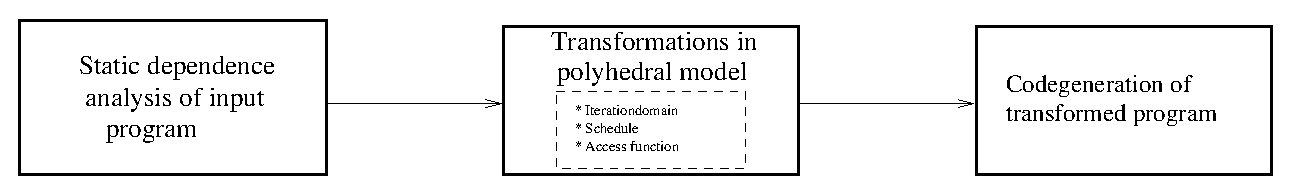
\includegraphics[width=1\textwidth]{images/poly_steps.eps}
  \caption{Transformation in polyhedral model}
  \label{fig:iter1}
\end{center}  
\end{figure}

\end{frame}

\begin{frame}[shrink]{Iteration domain}
\begin{columns}[t]
	\column{.5\textwidth}
	\begin{block}{ }
	{\tiny\lstinputlisting{listing6.tex}}
	\end{block}
	
	\column{.5\textwidth}
	\begin{block}{ }
	{\tiny\lstinputlisting{listing7.tex}}
	\end{block}
	\end{columns}
\pause
Iteration domain for {\textbf S1} is 
$D_{S1}\ =\ \{(i,j)\ \epsilon\ Z^2\ |\ 2\ \leq\ i\ \leq\ N\ \wedge\ 2\ \leq\ j\ \leq\ N\}$
\linebreak\linebreak
Iteration domain for {\textbf S2} is 
$D_{S2}\ =\ \{(i,j)\ \epsilon\ Z^2\ |\ 2\ \leq\ i\ \leq\ 6\ \wedge\ 2\ \leq\ j\ \leq\ 6\ \wedge\ i\ \leq\ j\}$
\pause
\begin{figure}
\begin{center}
  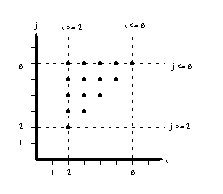
\includegraphics[height=5cm,width=5cm]{images/iter1.eps}
  \caption{Graphical representation of iteration domain(S2)}
  \label{fig:iter1}
\end{center}  
\end{figure}
\end{frame}

\begin{frame}{Schedule}
\begin{itemize}
\item Scattering function
\end{itemize}

\pause

\begin{block}{ }
{\tiny\lstinputlisting{listing8.tex}}
\end{block}
Examples: \\
$\phi_{S3}(i,j) = (i,j)$

$\phi_{S3}(i,j) = (j,i)$

\pause

\begin{block}{Code generated by Cloog for $\phi_{S3}(i,j) = (j,i)$}
{\tiny\lstinputlisting{listing9.tex}}
\end{block}


Loops are \textbf{\color{red}{interchanged}} here by applying this transformation
\end{frame}

\begin{frame}{Access function}
A[i+j][i+N]
\linebreak\linebreak
Array access function: $F_A(i,j) = (i+j,i+N)$ 
\linebreak\linebreak
{\textbf {\color{red}{Change array access function for better locality}}} \\
\end{frame}


\begin{frame}{SCoP - Static Control Part}
\begin{block}{Example for SCoP}
{\lstinputlisting{listing14.tex}}
\end{block}

\begin{itemize}
\item Structured control flow
	\begin{itemize}
	\item Regular for loops
	\item Conditions
	\end{itemize}
\item Affine expressions in:
	\begin{itemize}
	\item Loop bounds
	\item Conditions
	\item Access functions
	\end{itemize}
\item Side effect free(Pure functions)
\end{itemize}

\end{frame}

\begin{frame}{LLVM}
\begin{itemize}
\item LLVM (Low Level Virtual Machine)
	\begin{itemize}
	\item Framework for implementing compilers
	\item Common low level code repersentation
	\item Lifelong analysis and transformation of programs
	\end{itemize}
\end{itemize}
\end{frame}

\begin{frame}[allowframebreaks]{Polly}
\begin{itemize}
\item Polly (Polyhedral Optimization in LLVM)
	\begin{itemize}
	\item Implementing Polyhedral Optimization in LLVM
	\item Effort towards Auto Parallelism in programs.
	\end{itemize}
\item Implementation
	\begin{itemize}
	\item LLVM-IR to polyhedral model
			\begin{itemize}
			\item Region-based SCoP detection
			\item Semantic SCoPs
			\end{itemize}
	\item Polyhedral model
		\begin{itemize}
		\item The integer set library
		\item Composable polyhedral transformations
		\item Export/Import
		\end{itemize}
	\item Polyhedral model to LLVM-IR
	\end{itemize}
\item Related work
	\begin{itemize}
	\item gcc Graphite
	\end{itemize}
\end{itemize}

\begin{figure}
  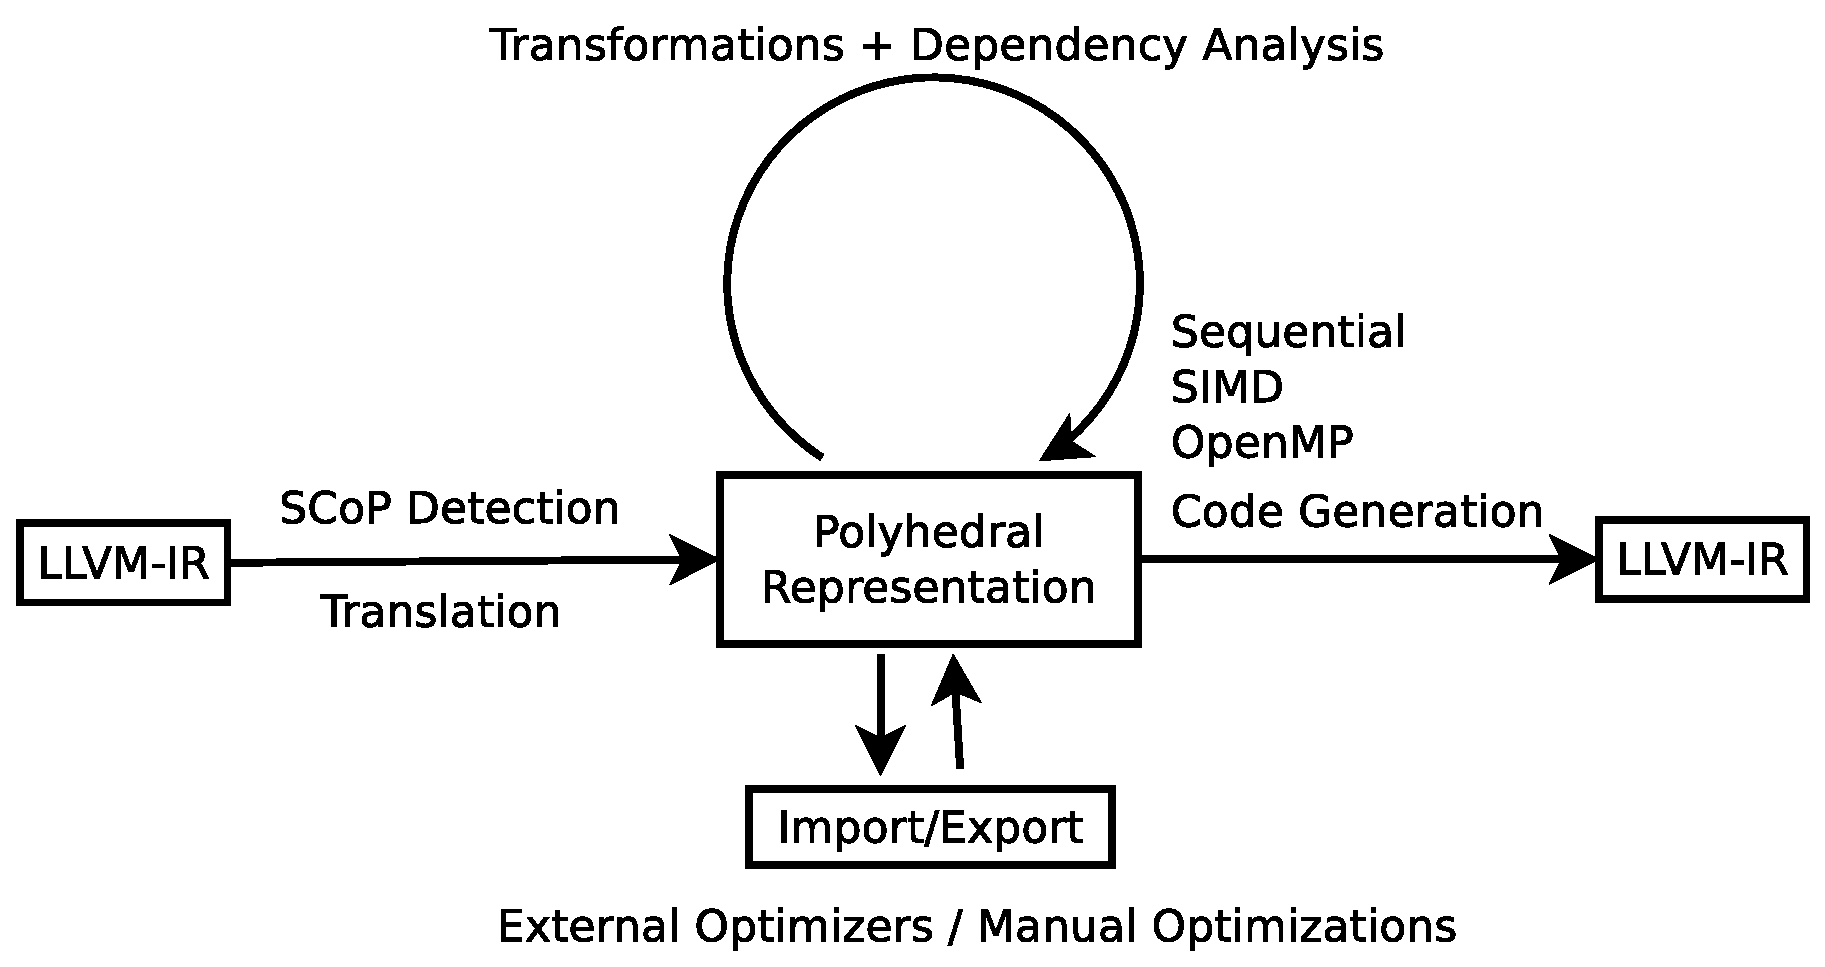
\includegraphics[width=1\textwidth]{images/architecture.eps}
  \caption{Architecture of Polly}
  \label{fig:arch}
\end{figure}
\end{frame}

\begin{frame}{OpenMP Code Generation in Polly}
\begin{figure}
\begin{center}
  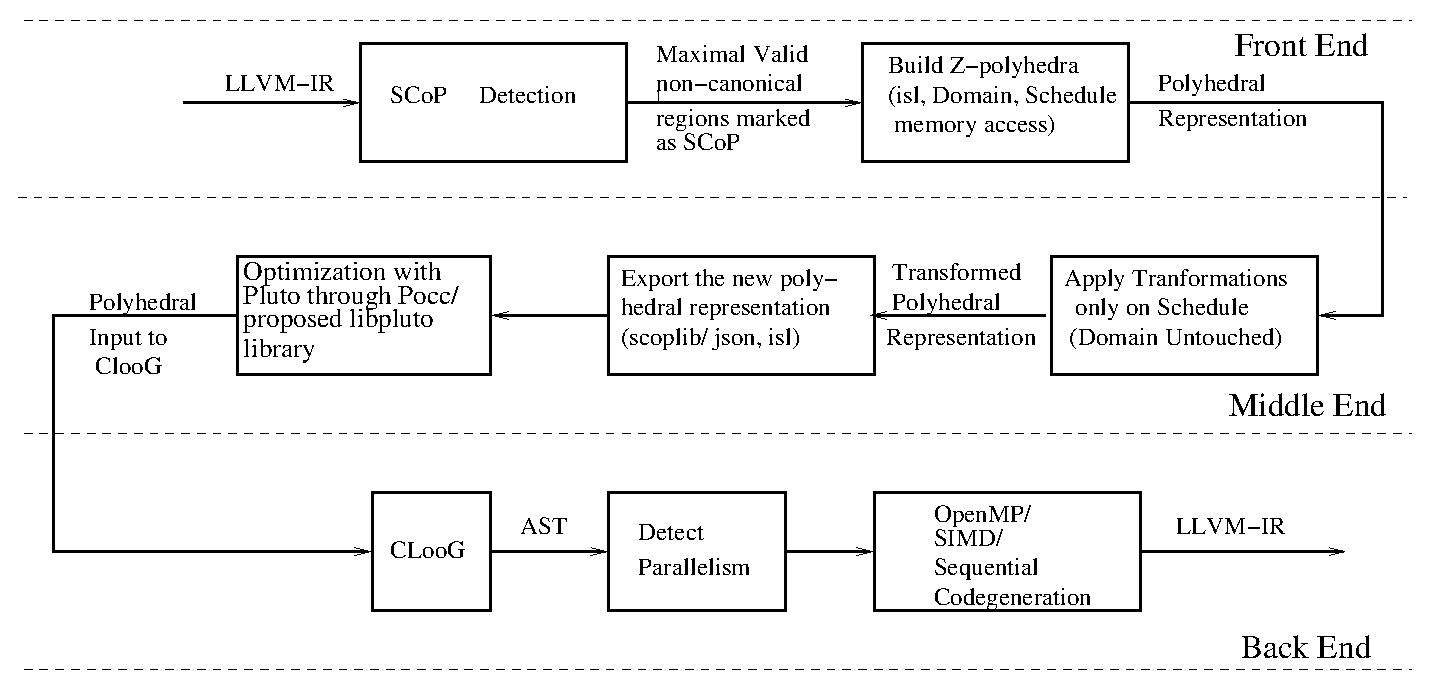
\includegraphics[width=1\textwidth]{images/detailedarch.eps}
  \caption{Detailed control flow in Polly}
  \label{detailed}
\end{center}
\end{figure}
\end{frame}


\begin{frame}{OpenMP Code Generation in Polly}
\begin{itemize}
\item Code generation pass in Polly
\item Detecting parallelism in Polly
\item Generating OpenMP library calls
\end{itemize}

\begin{block}{ }
{\tiny\lstinputlisting{listing10.tex}}
\end{block}
\end{frame}

\begin{frame}{OpenMP Code Generation in Polly}
\begin{figure}
  %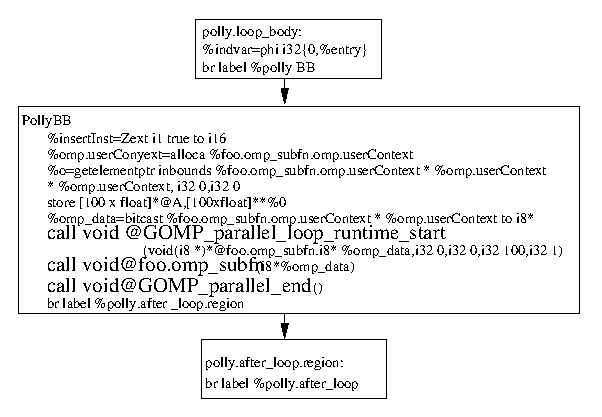
\includegraphics[width=1\textwidth]{images/ompcalls.eps}
  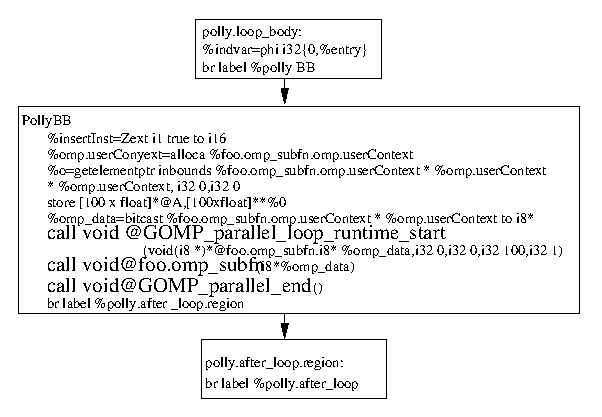
\includegraphics[width=1\textwidth]{images/ompcalls.eps}
  \caption{CFG showing sequence of OpenMP library calls}
  \label{fig:openmp_cfg}
\end{figure}
\end{frame}


\begin{frame}{OpenMP Code Generation in Polly}
\begin{itemize}
\item Support for inner loops

\begin{block}{ }
{\footnotesize\lstinputlisting{listing11.tex}}
\end{block}
Surrounding induction variables and parameters need to be passed to the subfunction
\pause
\item Dealing with memory references
\begin{block}{ }
{\footnotesize\lstinputlisting{listing12.tex}}
\end{block}
	\begin{itemize}
	\item Adding and extracting memory references
	\end{itemize}
\end{itemize}
\end{frame}


\begin{frame}{OpenMP Code Generation in Polly}
\begin{itemize}
\item Enabling OpenMP code generation in Polly
\begin{block}{ }
{\tiny\lstinputlisting{listing13.tex}}
\end{block}
\item OpenMP testcases
	\begin{itemize}
	\item Polly follows LLVM testing infrastrcutre
	\end{itemize}
\end{itemize}
\end{frame}

\begin{frame}{Testing with PolyBench}
\begin{itemize}
\item PolyBench \\
	\ \ \ Benchmarks from
	\begin{itemize}
	\item linear algebra
	\item datamining
	\item stencil computation
	\item solver and manipulation algorithms operating on matrices
	\end{itemize}
\end{itemize}
\end{frame}

\begin{frame}{Experimental results}
\begin{figure}
\begin{center}
  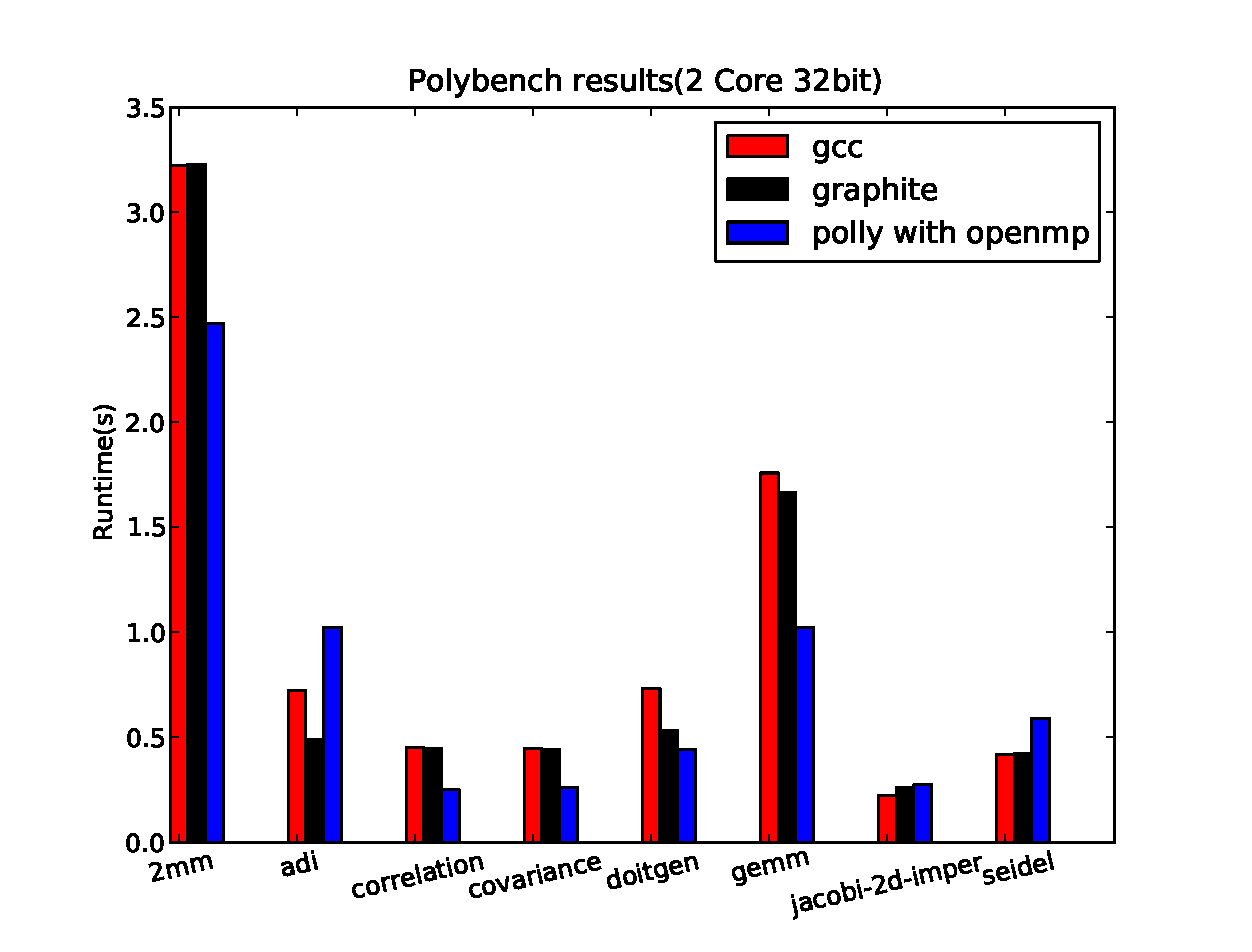
\includegraphics[height=7cm]{images/2core32bit.eps}
  \caption{Performance comparison(2 core 32 bit)}
  \label{fig:2core1}
\end{center}
\end{figure}
\end{frame}

\begin{frame}{Experimental results}
\begin{figure}
\begin{center}
  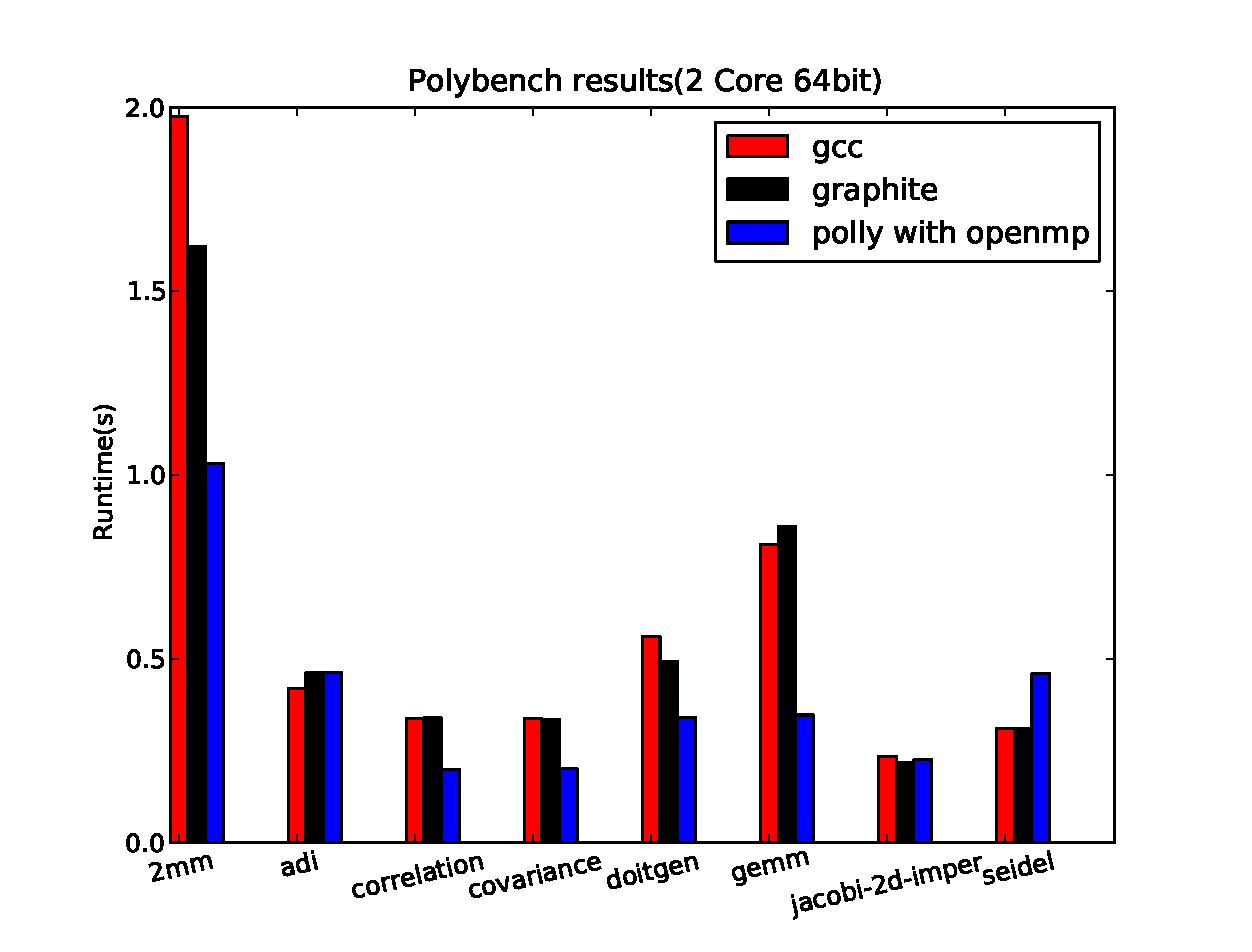
\includegraphics[height=7cm]{images/2core64bit.eps}
  \caption{Performance comparison(2 core 64bit)}
  \label{fig:2core2}
\end{center}
\end{figure}
\end{frame}

\begin{frame}{Experimental results}
\begin{figure}
\begin{center}
  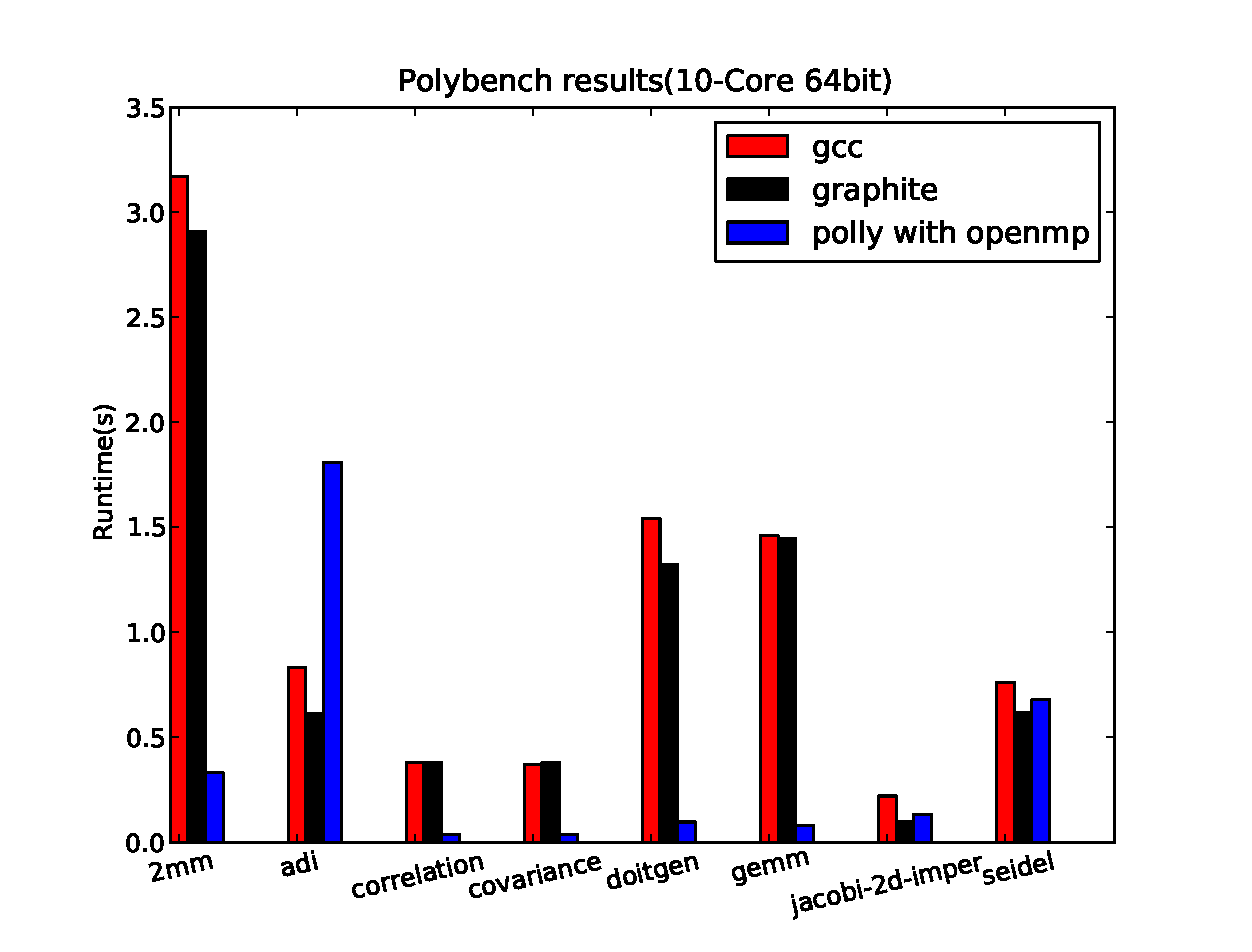
\includegraphics[height=7cm]{images/10core64bit.eps}
  \caption{Performance comparison(10-core 64 bit)}
  \label{fig:10core}
\end{center}
\end{figure}
\end{frame}

\begin{frame}{Conclusion and Future Work}
\begin{itemize}
\item Conclusion
\item Support for memory access transformations in Polly
\item Increasing coverage of Polly
	\begin{itemize}
	\item Increasing SCoP coverage
	\item Increasing the system coverage
	\end{itemize}
\item Integrating profile guided optimization into Polly
\end{itemize}
\end{frame}

\begin{frame}{Setting up the environment}
\begin{itemize}
\item CLooG
\item PoCC
\item Scoplib
\item Building LLVM with Polly
\end{itemize}
\end{frame}

\begin{frame}{Various Tools Used in Polyhedral Community}
\begin{itemize}
\item ClooG
\item PLUTO
\item VisualPolylib
\end{itemize}
\end{frame}

\end{document}
